\documentclass[11pt,aspectratio=169,handout]{beamer}

\usetheme{Singapore}
\usecolortheme{orchid}

\usepackage[utf8]{inputenc}
\usepackage[russian]{babel}
\usepackage{amsmath}
\usepackage{amsfonts}
\usepackage{amssymb}
\usepackage{graphicx}
\usepackage{bibentry}
\usepackage{wasysym}
\usepackage[most]{tcolorbox}
\usepackage[normalem]{ulem}

\usepackage{hyperref}

\definecolor{info}{RGB}{62, 180, 137}
\definecolor{warn}{RGB}{128, 0, 0}

\author{Сергей Малышев}
\title{Большие рекомендательные модели}
\date{16 апреля 2025 г.}

\AtBeginSection[]{
  \begin{frame}
  \vfill
  \centering
  \begin{beamercolorbox}[sep=8pt,center,shadow=true,rounded=true]{title}
    \usebeamerfont{title}\insertsectionhead\par
  \end{beamercolorbox}
  \vfill
  \end{frame}
}

\logo{
\includegraphics[width=.05\textwidth]{images/ok_logo.png}}


\begin{document}

{
\setbeamertemplate{headline}{}

\begin{frame}
\titlepage
\end{frame}

%\begin{frame}
%\tableofcontents
%\end{frame}

}

\begin{frame}{Контекст}

\begin{center}
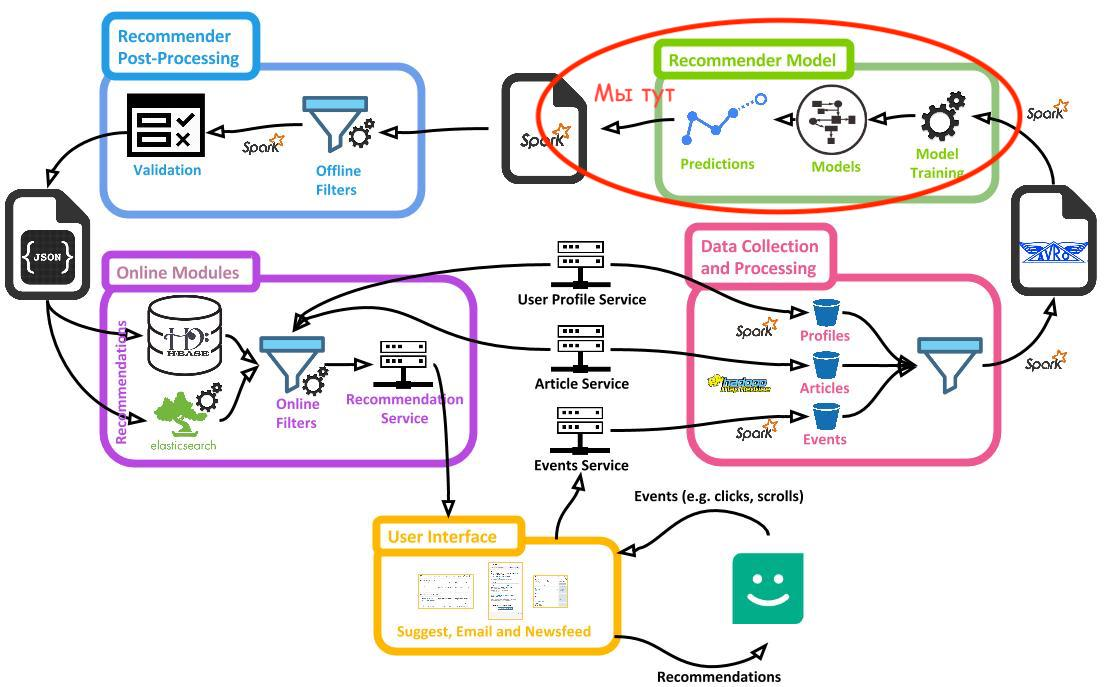
\includegraphics[scale=0.23]{images/mendeley.jpeg}
\end{center}

\end{frame}

\section{Мотивация}

\begin{frame}{Какие сейчас проблемы у стандартных рекомендательных моделей?}
\begin{center}
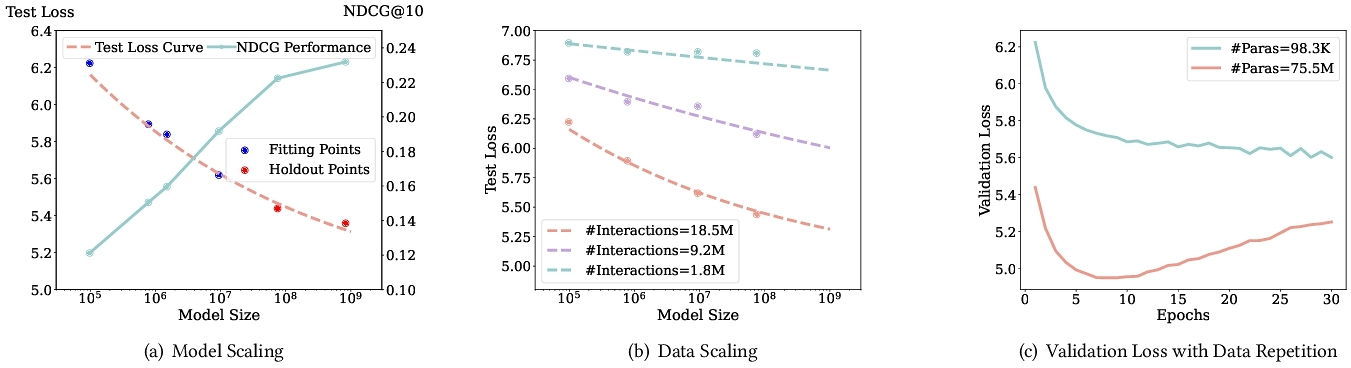
\includegraphics[scale=0.7]{images/scaling_law_large_seq_recs.jpg}
\end{center}


\vfill
\begin{small}
\begin{tabular}{l l}
Проблема №1: & Не можем запихнуть все айтемы в одну модель \\
Проблема №2: & Качество моделей перестает расти при увеличении \\
& параметров\cite{zhang2024scaling} / размера датасета

\end{tabular}
\end{small}

\textbf{

}
\end{frame}

\begin{frame}{Чего мы хотим?}
\begin{center}
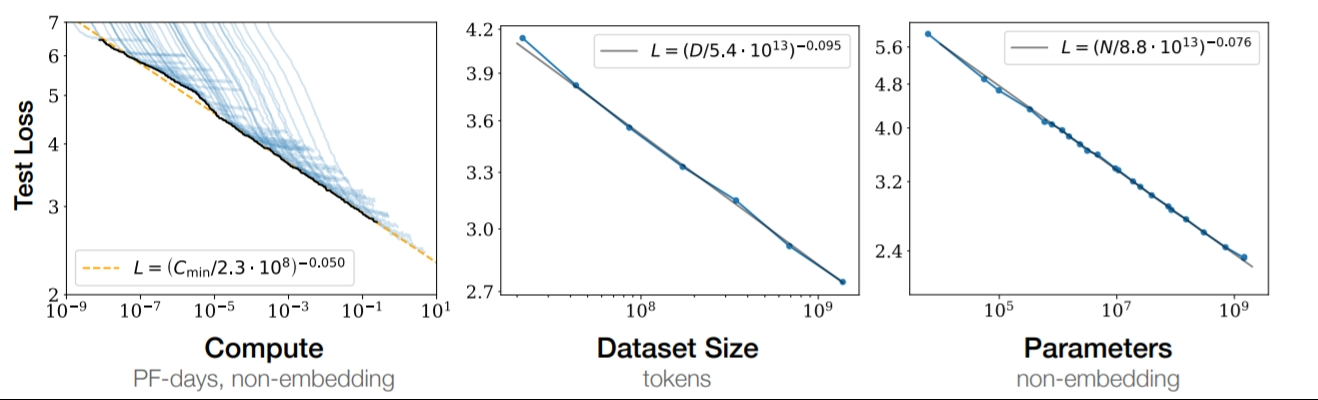
\includegraphics[scale=0.25]{images/scaling_laws.png}
\end{center}

\vfill
\begin{small}
\begin{tabular}{l l}
Потребность №1: & Хотим передавать все айтемы в модель \\
Потребность №2: & Хотим растить качество модели на уровне линейного роста по мере роста \\
& датасета / увеличения количества параметров
\footnote{\url{ttps://www.lesswrong.com/w/scaling-laws}}
\end{tabular}
\end{small}

\end{frame}


\section{Архитектуры больших рек. моделей}

\begin{frame}{Deep Learning Recommendation Model for Personalization and Recommendation Systems \cite{naumov2019deep}}

\begin{columns}
\begin{column}{0.5\textwidth} 
\begin{center}
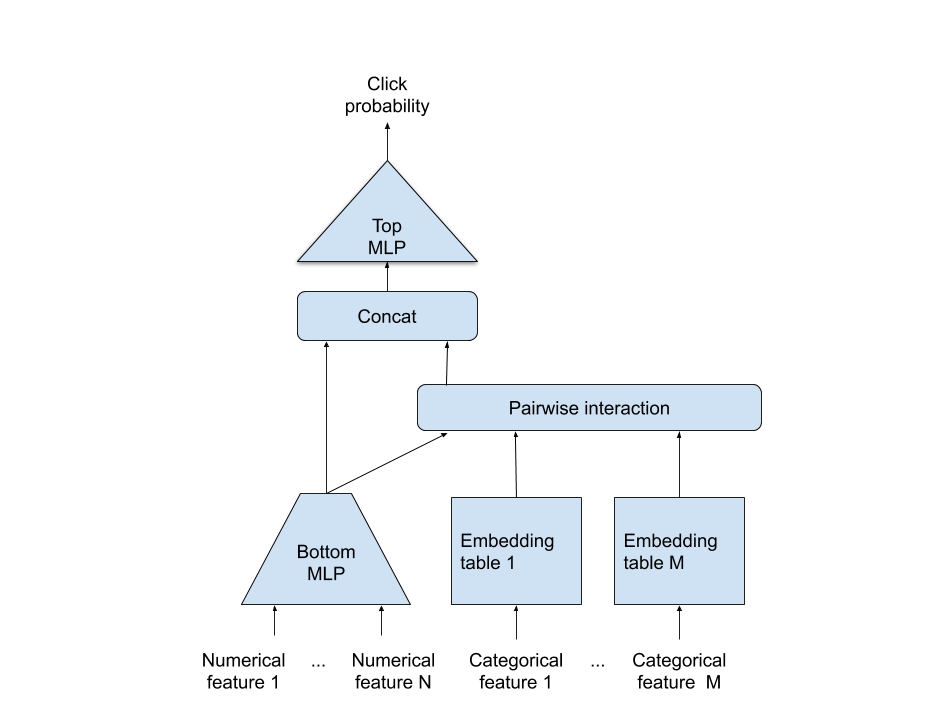
\includegraphics[scale=0.2]{images/dlrm-arch.png}
\end{center}
\end{column}
\begin{column}{0.5\textwidth}
\begin{center}
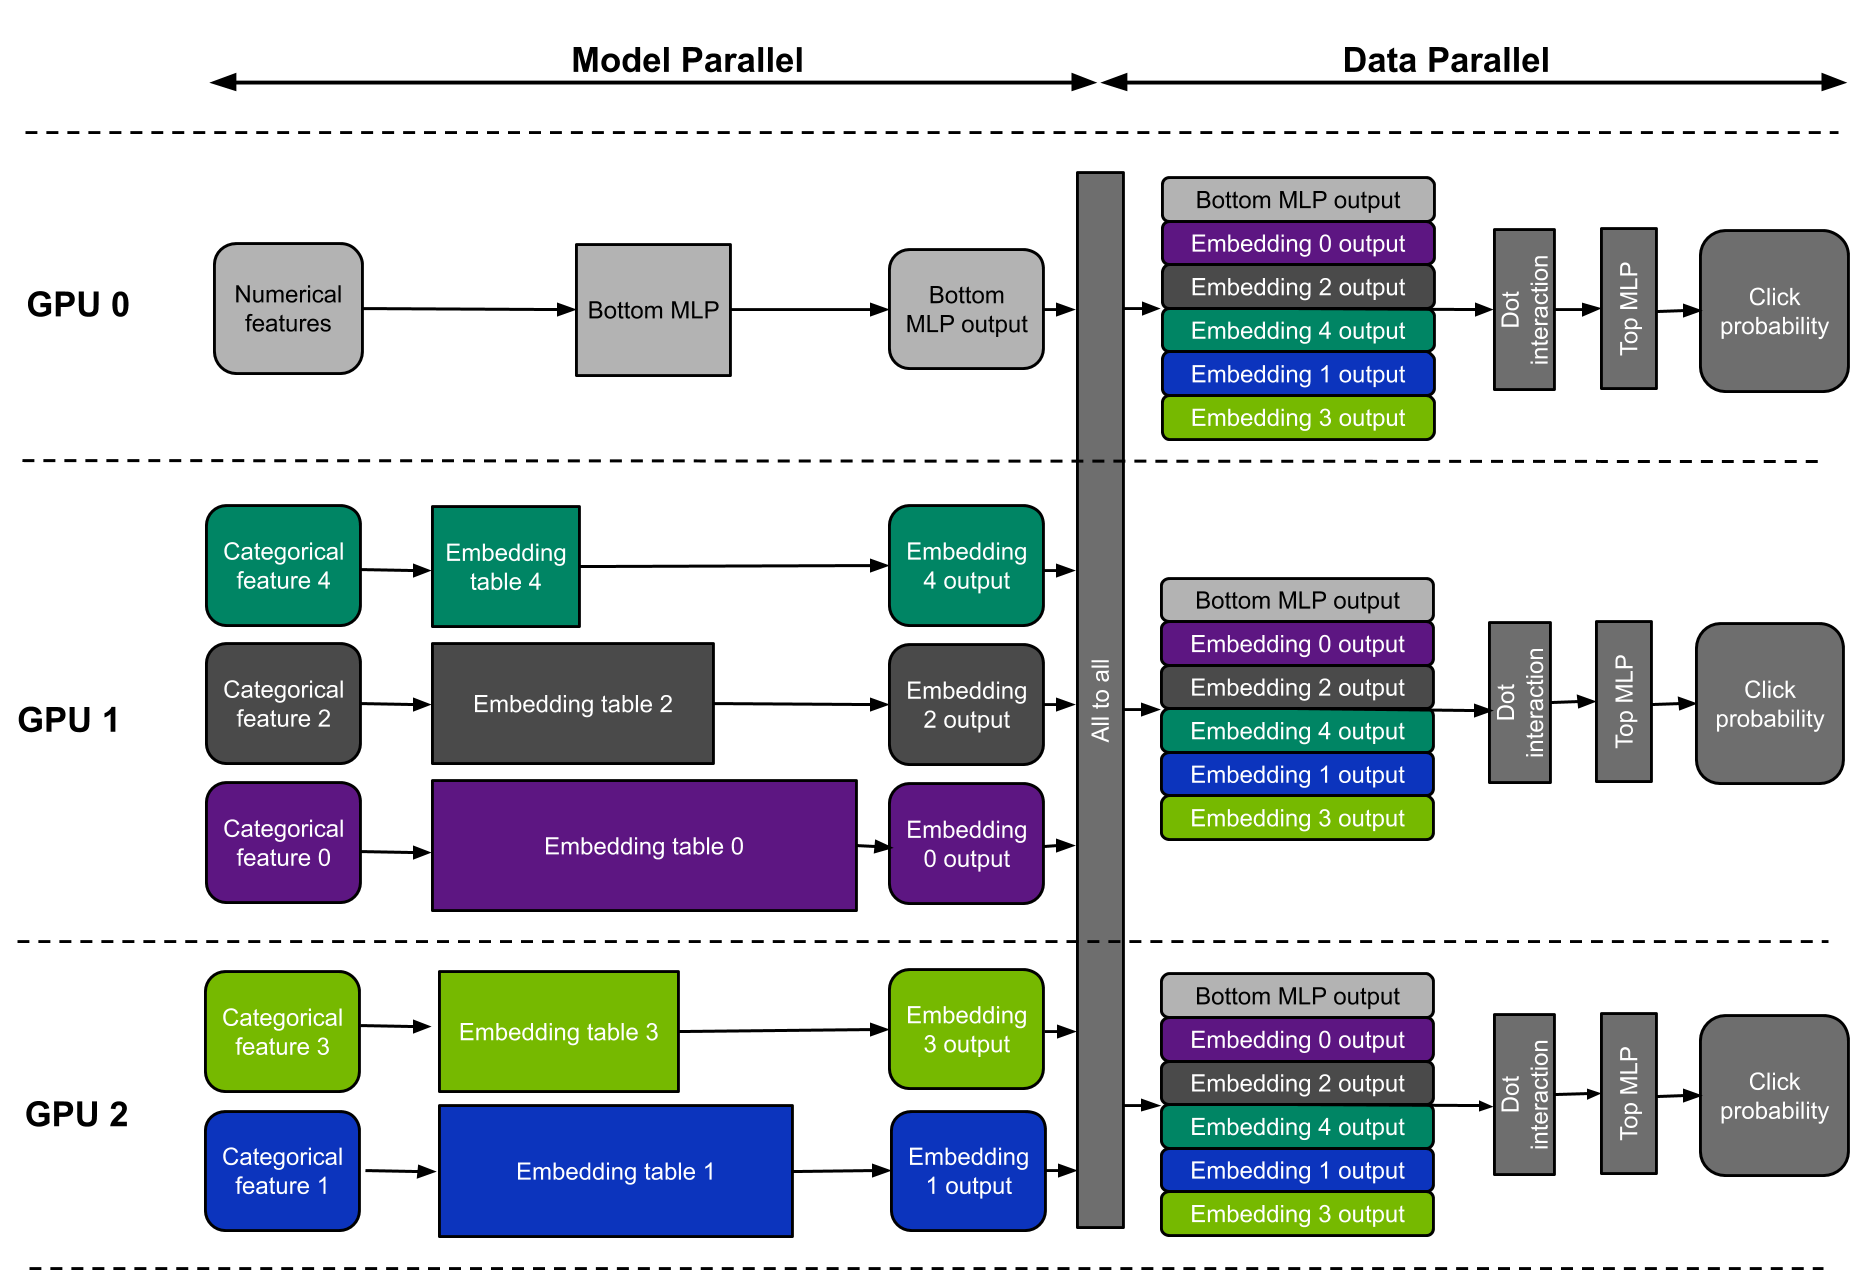
\includegraphics[scale=0.1]{images/dlrm-parallel.png}
\end{center}
\end{column}
\end{columns}

\vfill
\begin{small}
\begin{tabular}{l l}
Идея & Простая архитектура, но много параметров в эмбеддингах\footnote{\url{https://catalog.ngc.nvidia.com/orgs/nvidia/resources/dlrm_for_pytorch}}
\end{tabular}
\end{small}

\end{frame}

\begin{frame}{Semantic ID \cite{singh2024better}}

\begin{center}
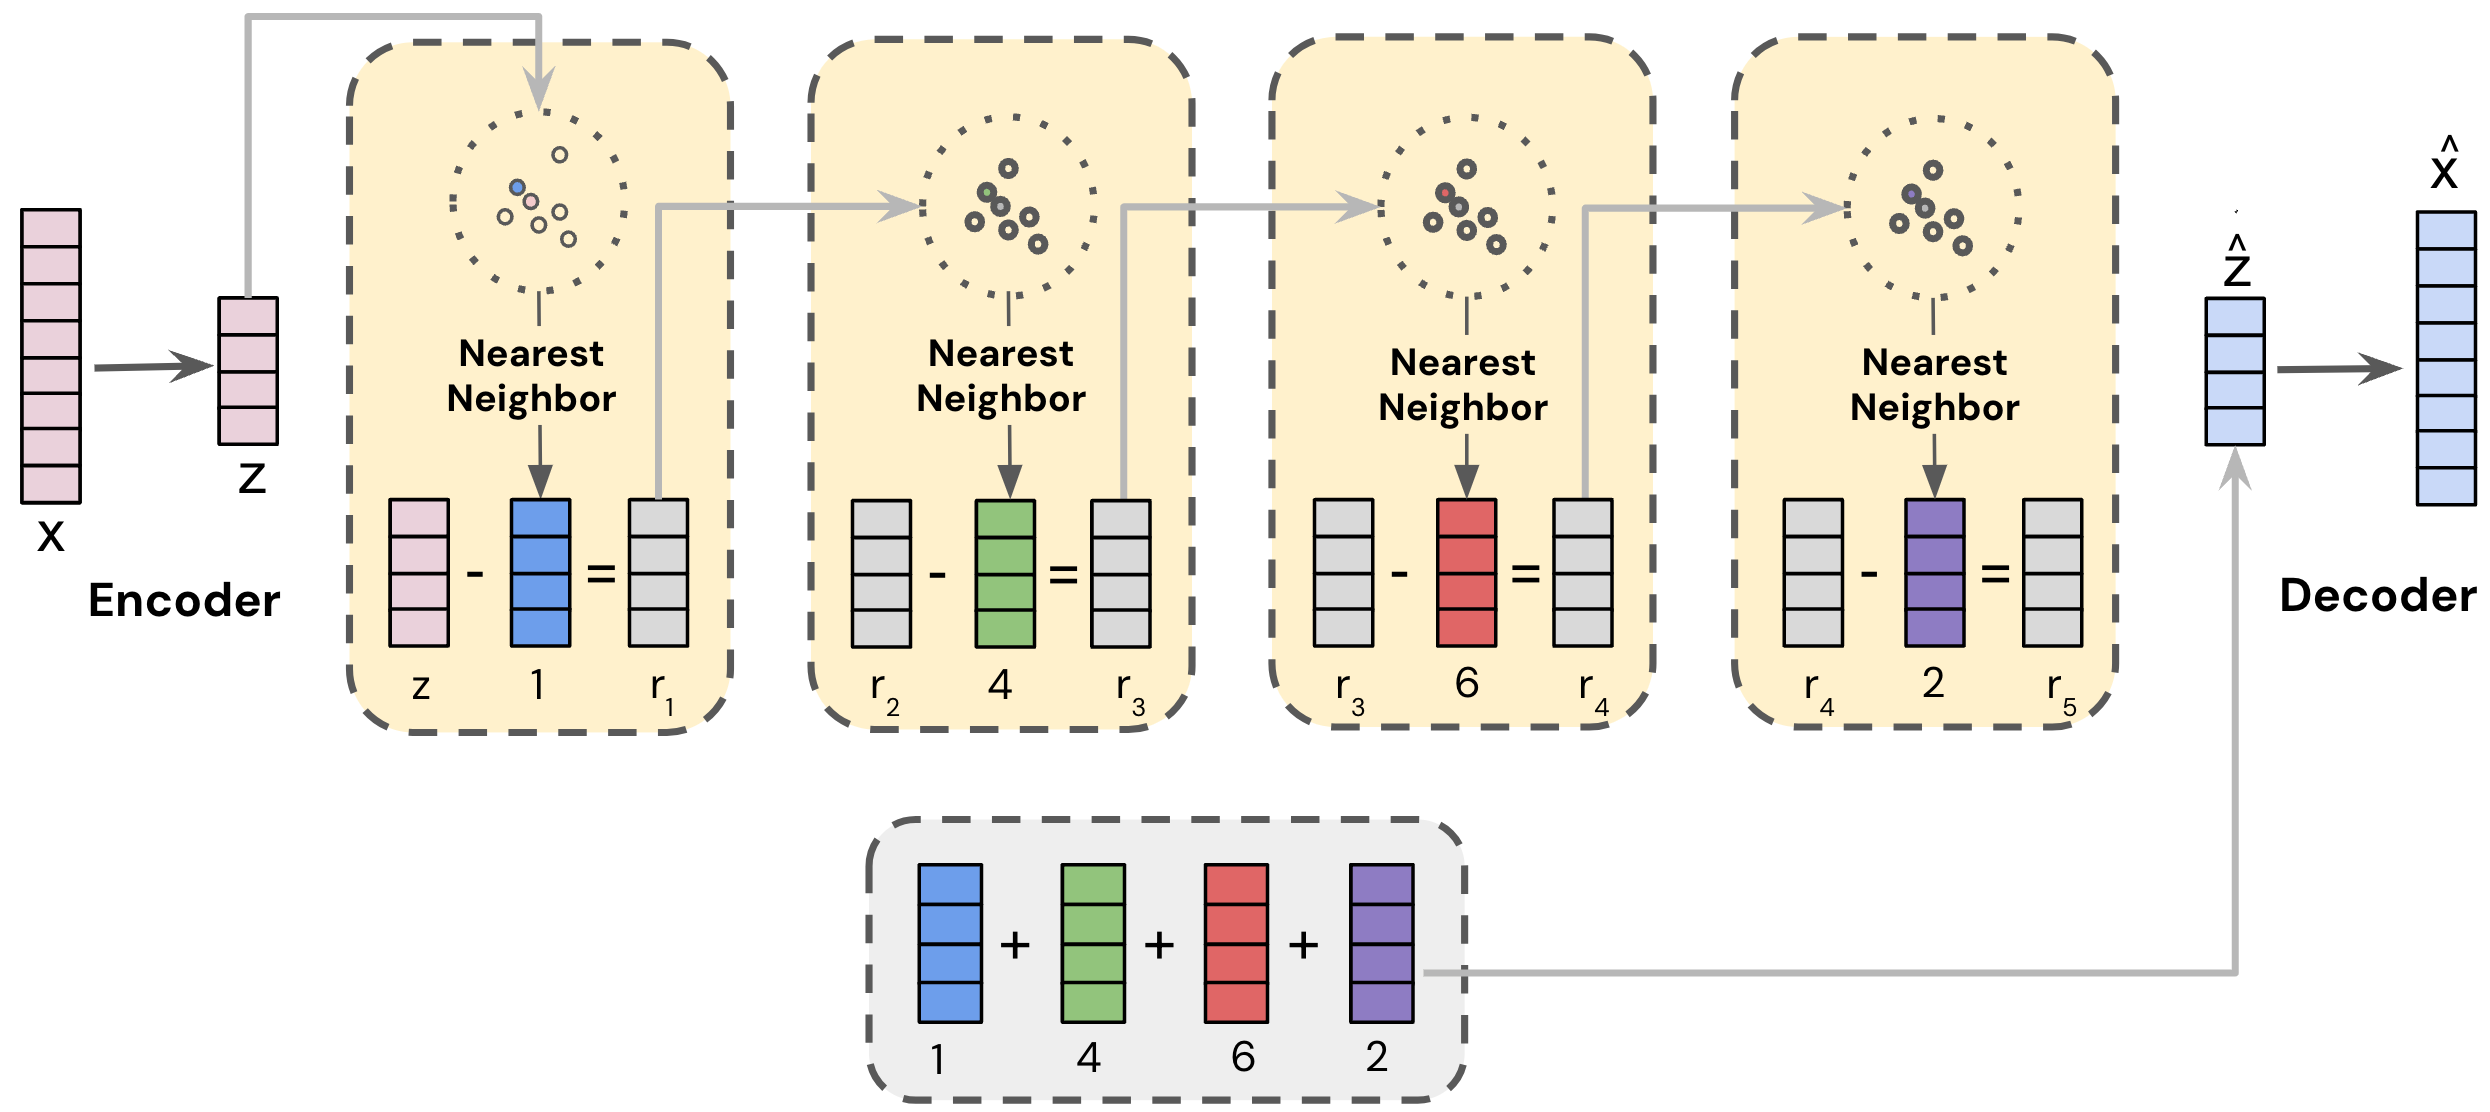
\includegraphics[scale=0.1]{images/rqvae_sid_spm.png}
\end{center}

\vfill
\begin{small}
\begin{tabular}{l l}
Идея & * С помощью RQ VAE кодируем айтемы последовательностью целых чисел \\
& * Используем как эмбеддинг для другой модели \\
& * Решаем проблему холодного старта
\end{tabular}
\end{small}

\end{frame}

\begin{frame}{Recommender Systems with Generative Retrieval \cite{rajput2023recommender}}

\begin{columns}
\begin{column}{0.5\textwidth} 
\begin{center}
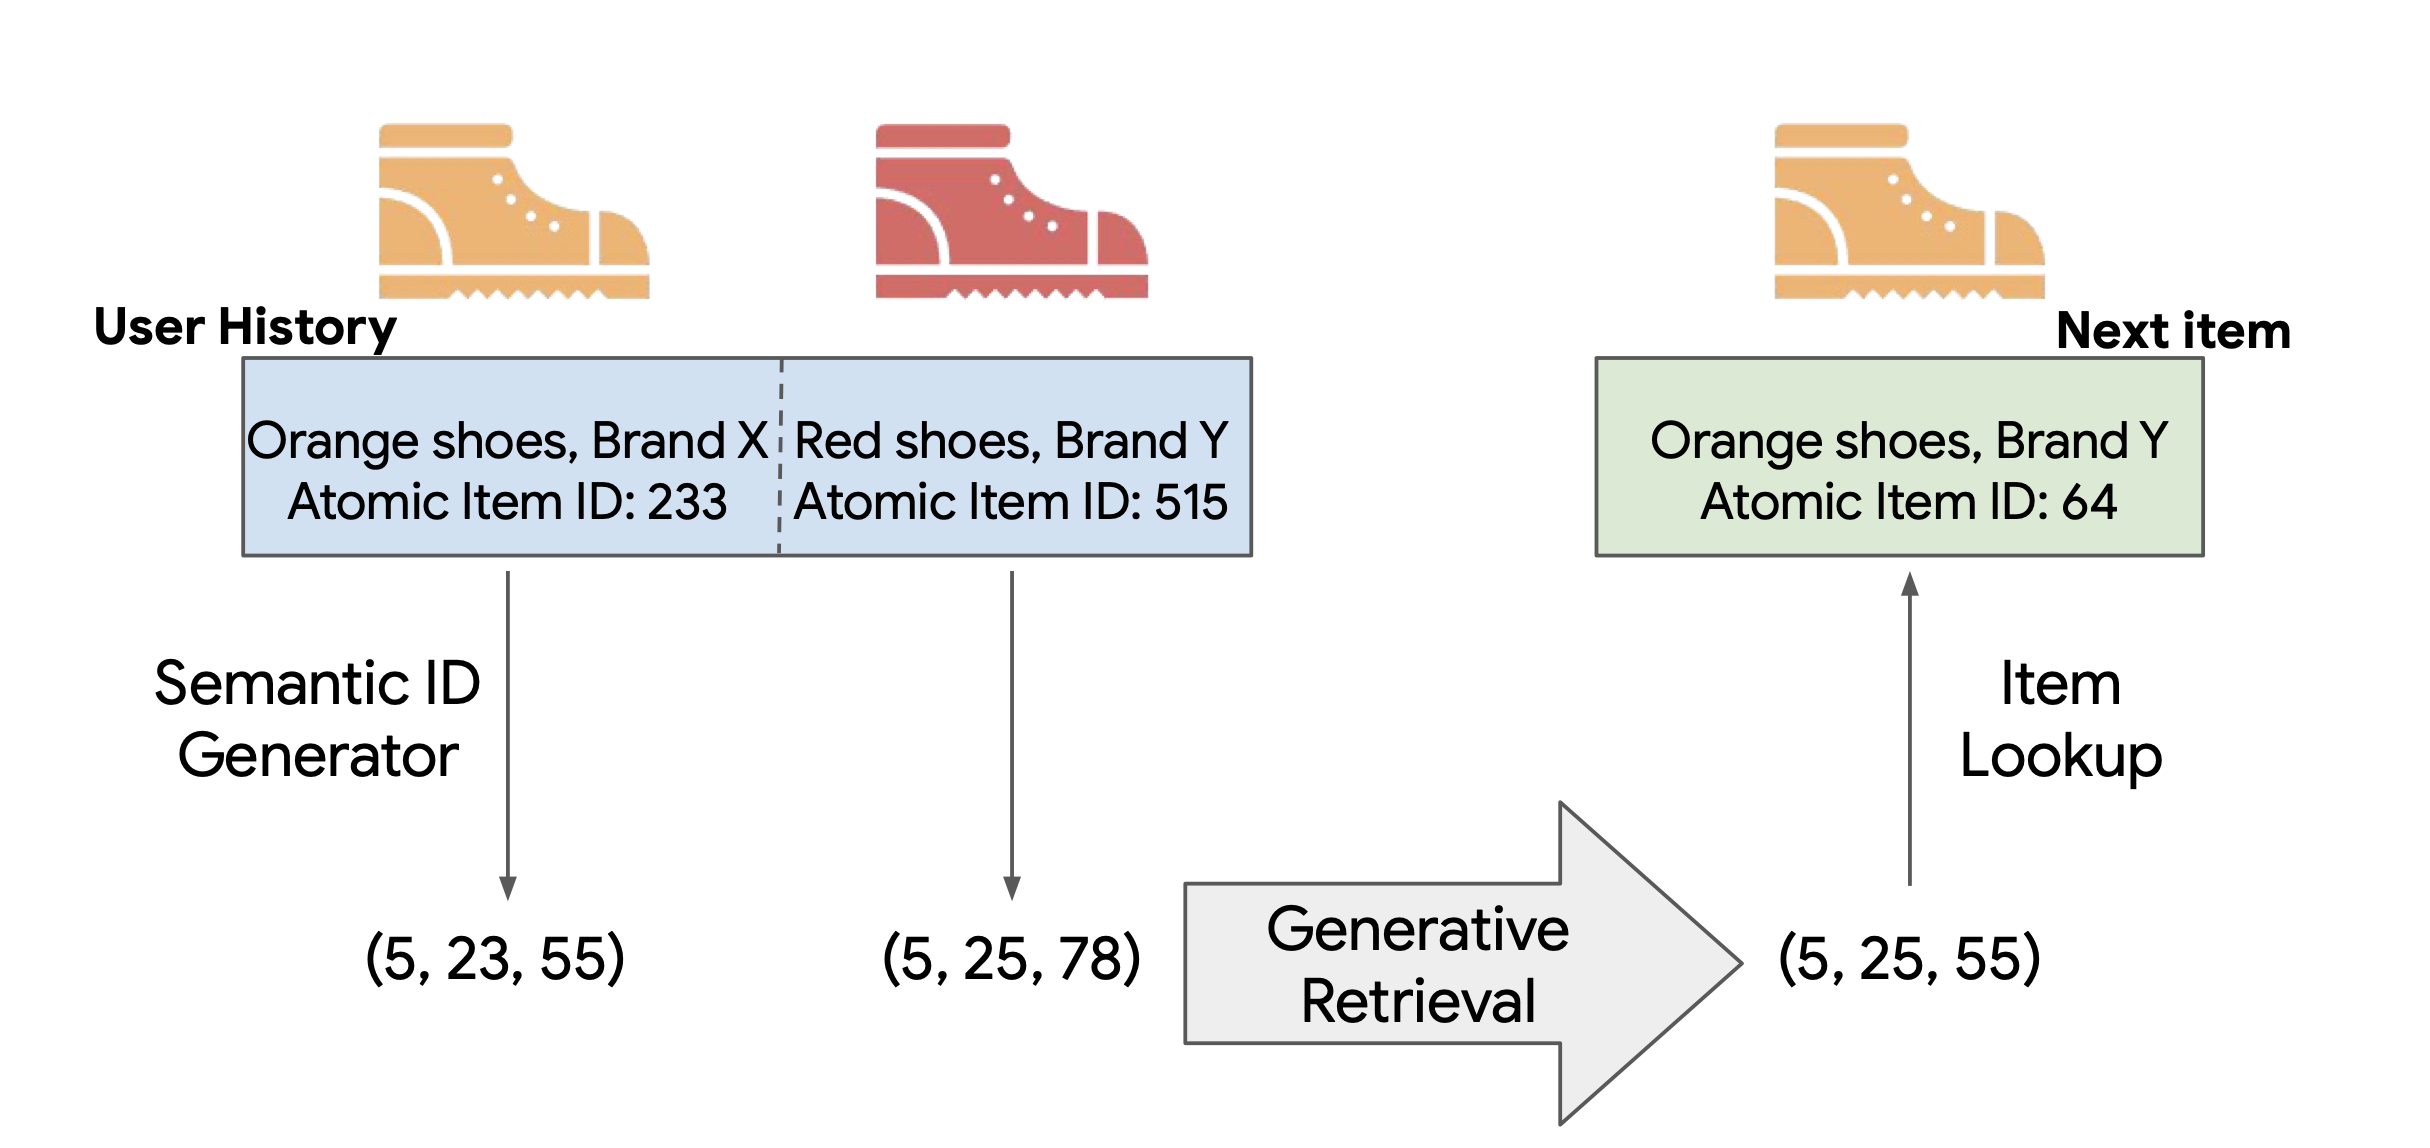
\includegraphics[scale=0.15]{images/semantic_ids_seq.png}
\end{center}
\end{column}
\begin{column}{0.5\textwidth}
\begin{center}
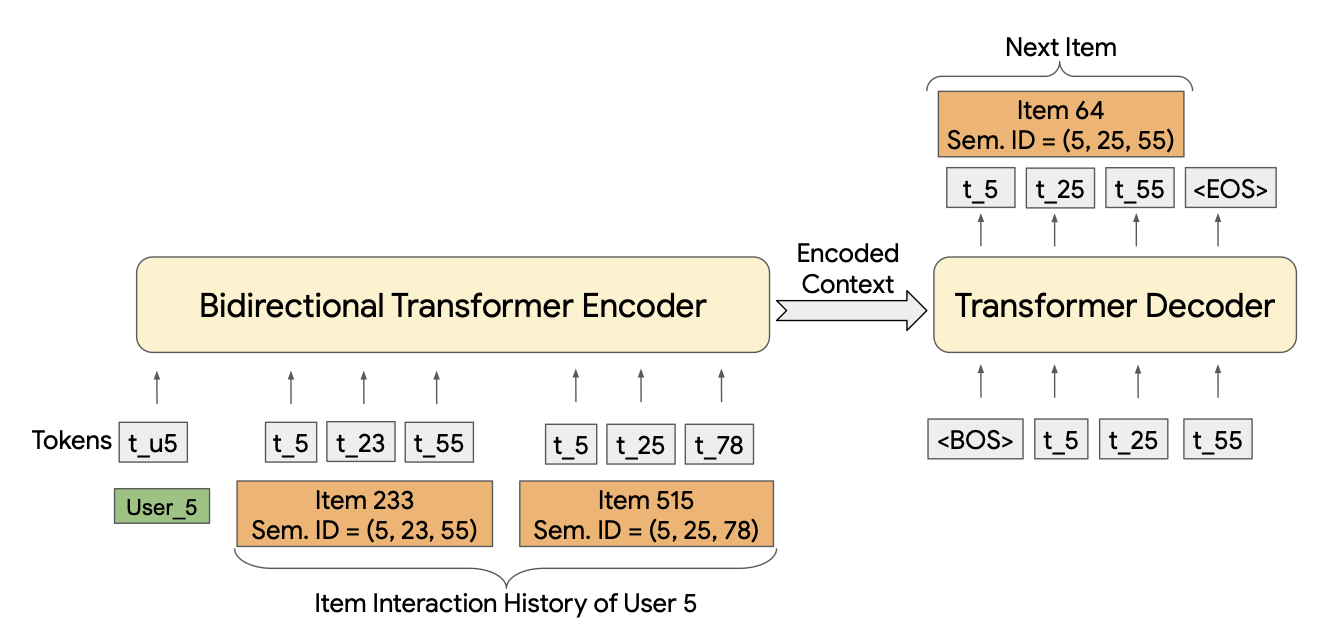
\includegraphics[scale=0.3]{images/encoder_decoder_semantic.png}
\end{center}
\end{column}
\end{columns}

\vfill
\begin{small}
\begin{tabular}{l l}
Идея & * Строим seq2seq модель из Semantic-IDs получая end2end подход\\
& * Решаем проблему холодного старта\\
& * Делаем рекомендации разнообразнее
\end{tabular}
\end{small}

\end{frame}


\begin{frame}{HSTU \cite{zhai2024actions}}

\begin{columns}
\begin{column}{0.5\textwidth} 
\begin{center}
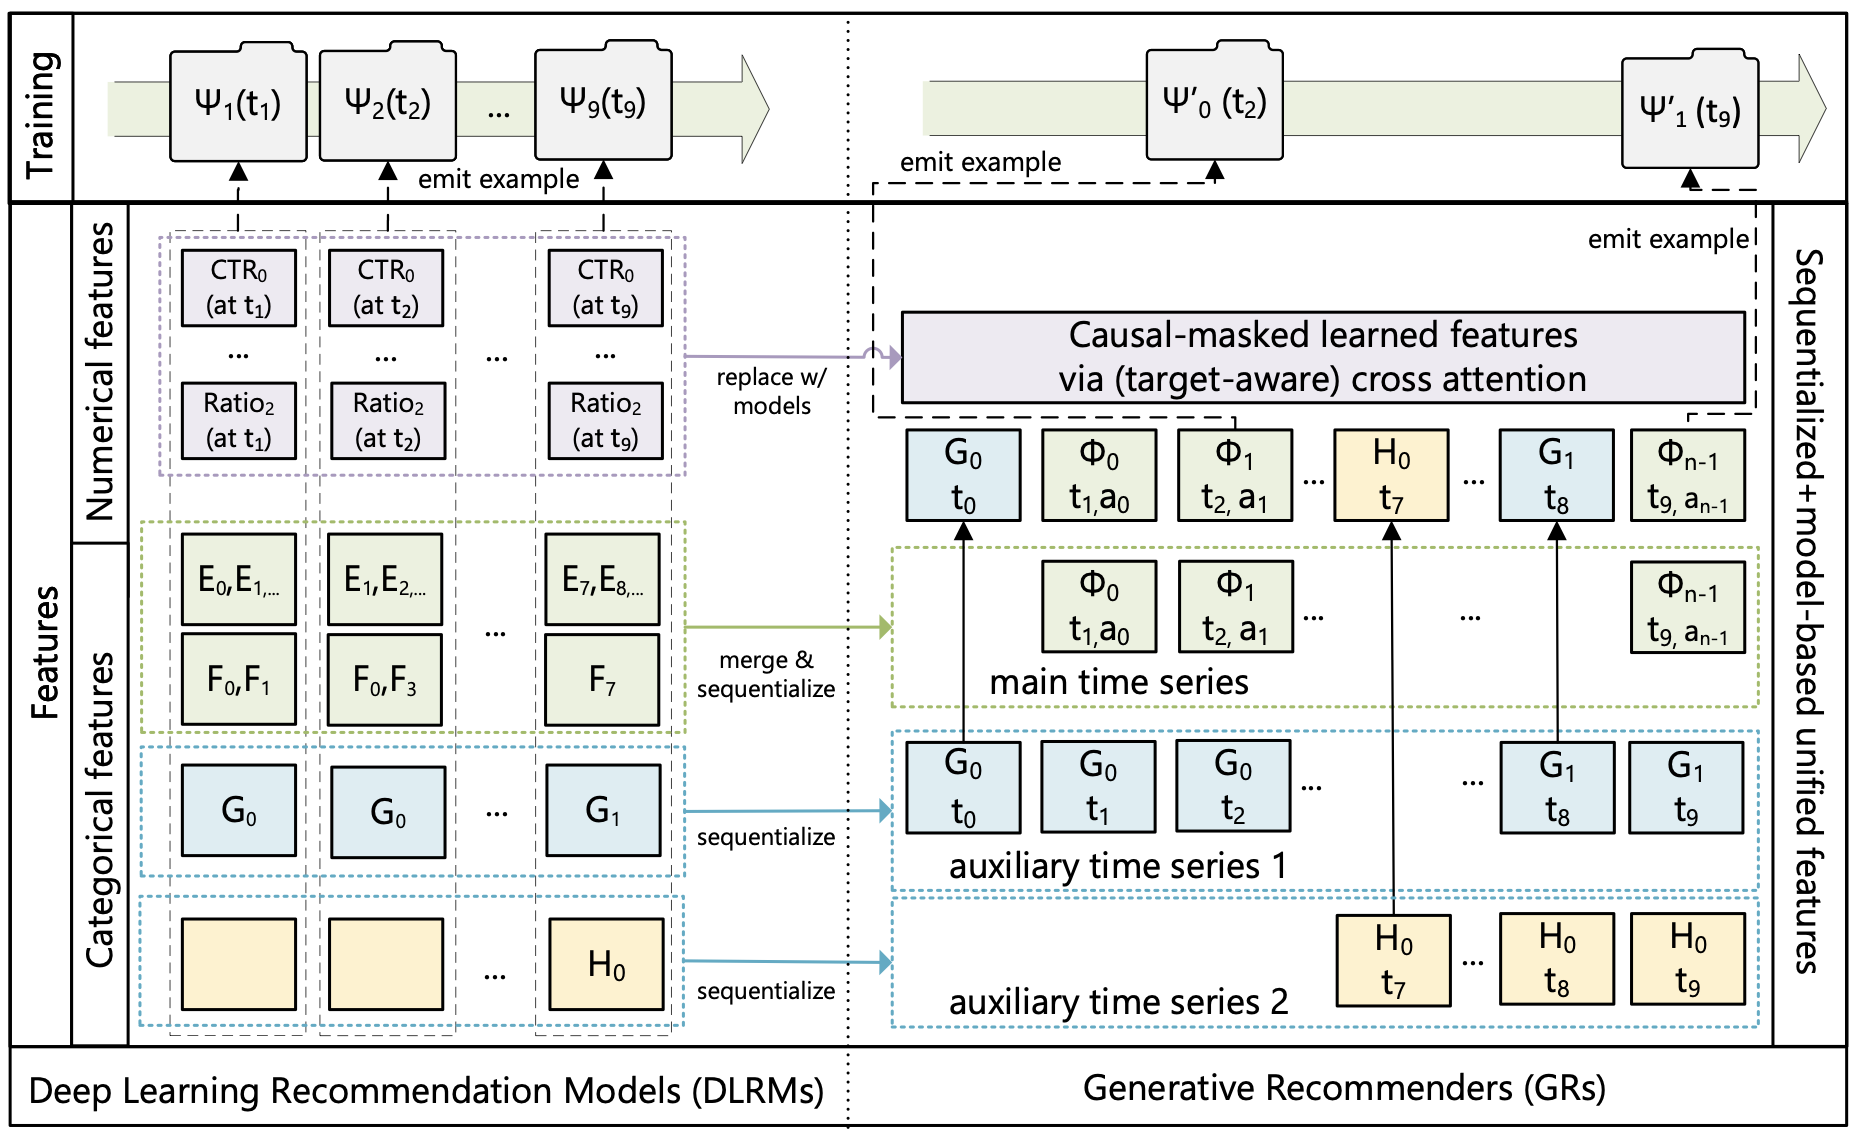
\includegraphics[scale=0.20]{images/hstu_arch.png}
\end{center}
\end{column}

\begin{column}{0.5\textwidth}
\begin{center}
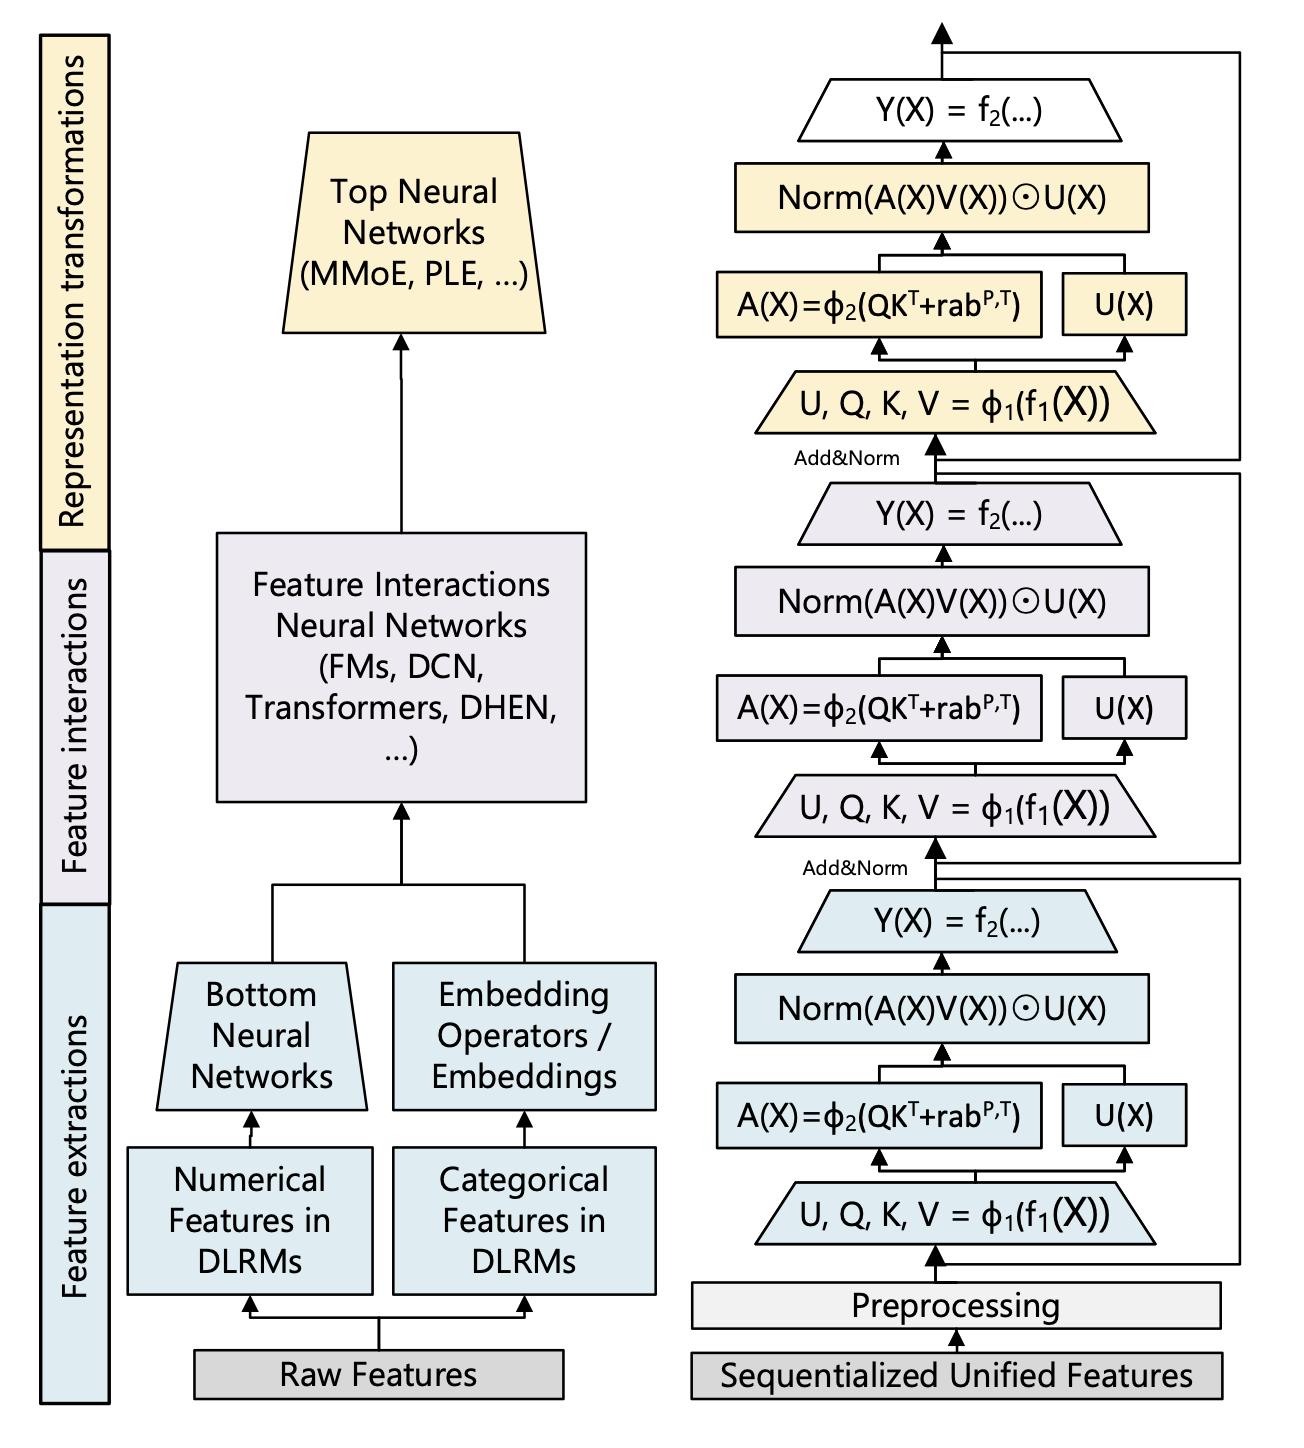
\includegraphics[scale=0.20]{images/hstu_block.png}
\end{center}
\end{column}
\end{columns}

\vfill
\begin{small}
\begin{tabular}{l l}
Идея & * Меняем постановку на генеративную\\
& * Используем изменения контекста\\
& * Вместо фичей используем экшены пользователей\\
& * Вместо DLRM используем HSTU блок с attention без FFN
\end{tabular}
\end{small}
\end{frame}


\begin{frame}{FuXi-alpha \cite{ye2025fuxi}}

\begin{columns}
\begin{column}{0.5\textwidth} 
\begin{center}
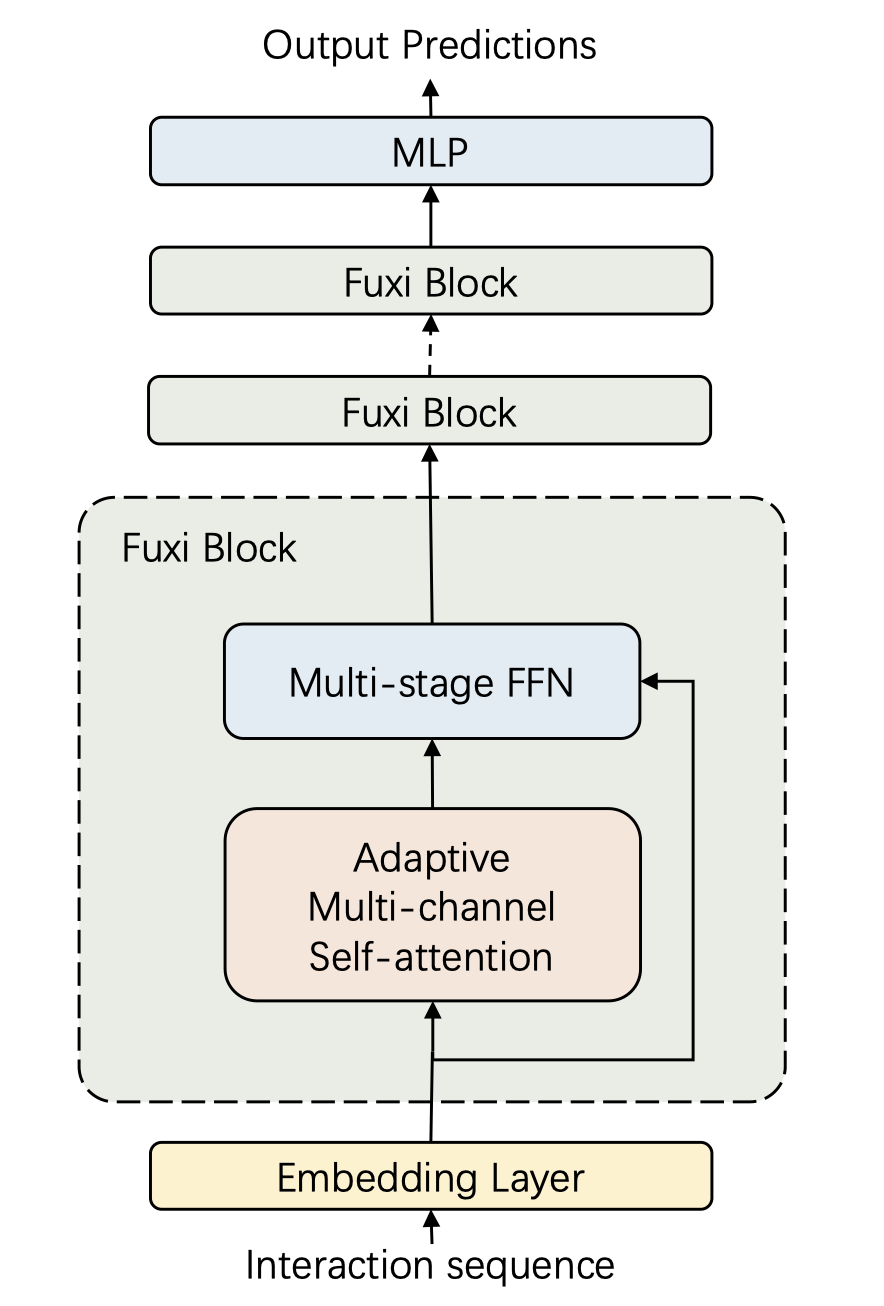
\includegraphics[scale=0.25]{images/fuxi-alpha-arch.png}
\end{center}
\end{column}

\begin{column}{0.5\textwidth}
\begin{center}
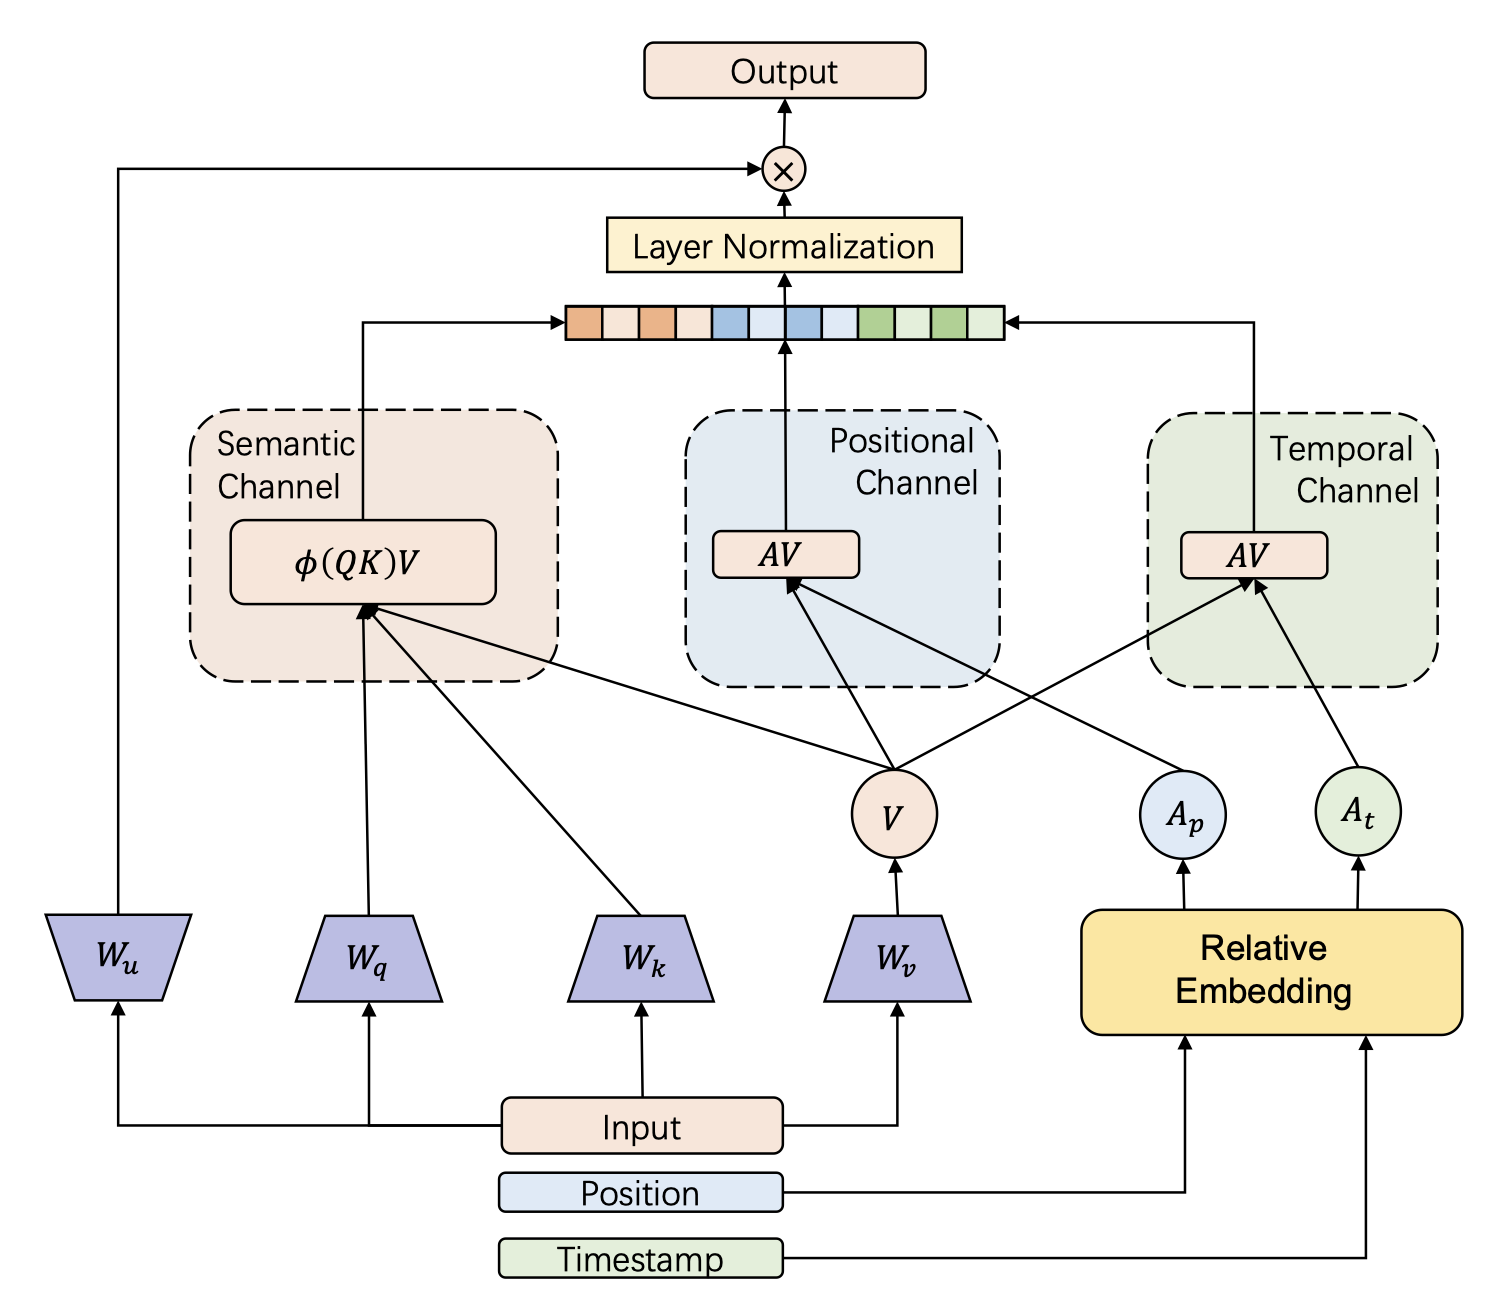
\includegraphics[scale=0.25]{images/fuxi-alpha-ams.png}
\end{center}
\end{column}
\end{columns}

\vfill
\begin{small}
\begin{tabular}{l l}
Идея & * Берем HSTU за основу\\
& * Возвращаем туда FFN\\
& * Cвои механизмы attention для позиционной и темпоральной компоненты
\end{tabular}
\end{small}
\end{frame}


\begin{frame}{Немного про метрики и масштабируемость}

\begin{center}
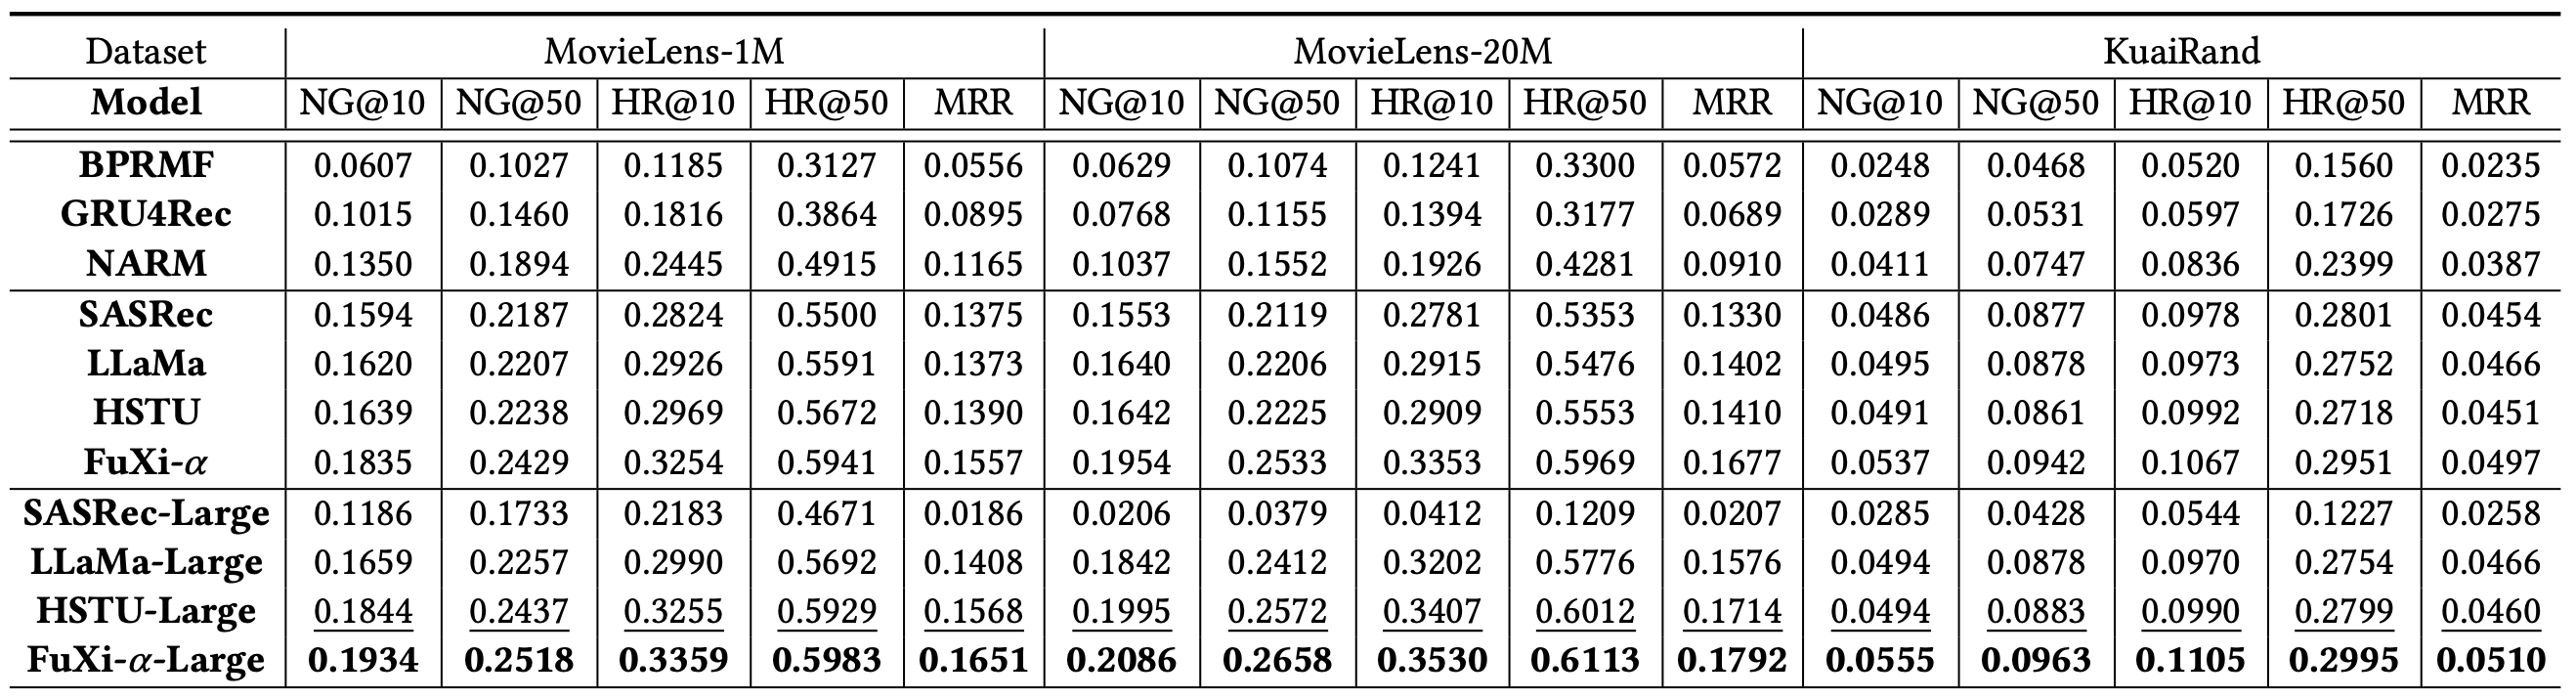
\includegraphics[scale=0.3]{images/fuxi_alpha_metrics.png}
\end{center}

\end{frame}

\begin{frame}{360Brew \cite{firooz2025360brew}}

\begin{center}
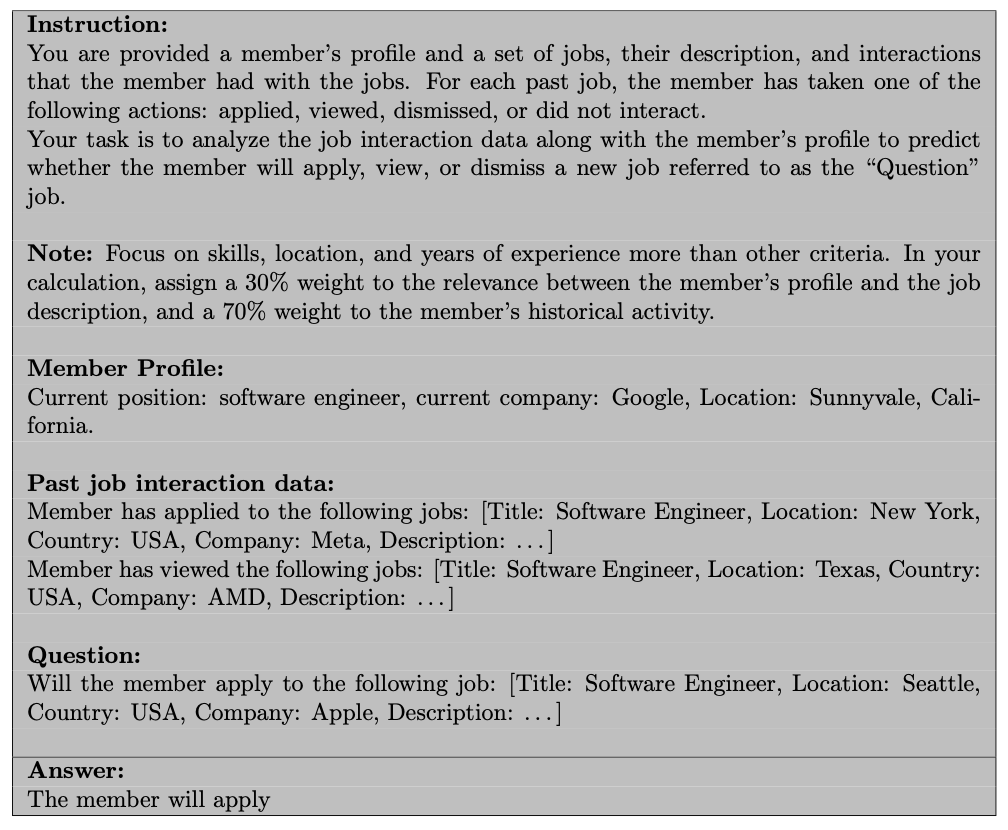
\includegraphics[scale=0.4]{images/360brew_input.png}
\end{center}

\vfill
\begin{small}
\begin{tabular}{l l}
Идея & * Дообучаем предобученную LLM-ку Mixtral на постановку рекомендаций\\
& * Continuous pretraining, instruction fine-tuning, supervised fine-tuning
\end{tabular}
\end{small}

\end{frame}


\section{Итоги}

\begin{frame}{Итоги}

\begin{tcolorbox}[colback=info!5,colframe=info!80,title=]
Плавненько движемся в сторону генеративной постановки рекомендаций по аналогии с LLM
\end{tcolorbox}

\begin{tcolorbox}[colback=warn!5,colframe=warn!80,title=]
А так же в сторону foundation моделей
\end{tcolorbox}

\begin{tcolorbox}[colback=warn!5,colframe=warn!80,title=]
Получаем за счет этого буст по качеству
\end{tcolorbox}

\begin{tcolorbox}[colback=warn!5,colframe=warn!80,title=]
Попутно решаем проблему холодного старта
\end{tcolorbox}

\begin{tcolorbox}[colback=warn!5,colframe=warn!80,title=]
Но пока все это есть лишь у единиц, подходы должны настояться
\end{tcolorbox}

\end{frame}

\begin{frame}{До следующего раза \cite{zhai2024actions}}

\begin{columns}
\begin{column}{0.45\textwidth}
   \begin{center}
                
\includegraphics[scale=0.35]{images/bye.png}
   \end{center}
\end{column}
\begin{column}{0.45\textwidth}
   \begin{center}
                \url{https://t.me/mlvok}

                
\includegraphics[scale=0.5]{images/tgqr.png}
   \end{center}
\end{column}
\end{columns}

\end{frame}

\begin{frame}[allowframebreaks]{Литература}

\bibliographystyle{amsalpha}
\bibliography{references}

\end{frame}


\end{document}
